%%% OPERA: Robust Representation Learning for Irregular Time Series under Observation-Process Shift
%%%
%%% MAIN DRIVER. This file holds the preamble and front matter only; every section lives in sections/ and is
%%% pulled in with \input below. Compile this file (not main.tex, which has been retired):
%%%
%%%     latexmk -pdf sigconf.tex          % or select sigconf.tex as the main document in Overleaf
%%%
%%% Conventions:
%%%   \prelim (dagger) marks a number obtained from a single seed. The protocol requires five.
%%%   \todo{...} marks a pending measurement. Do not delete either marker without replacing the number.
%%%   Numbers come from results/raw/*/results.json via results/aggregated/tables_<dataset>.md.
%%%
%%% NOTE ON MATH PACKAGES: do not add amsmath or amssymb. Under XeLaTeX/LuaLaTeX acmart already loads
%%% amssymb + unicode-math, and requesting amssymb here raises "Command \Bbbk already defined". The sections
%%% deliberately avoid amsmath-only constructs (align, \boxed, \text), so this compiles under pdfLaTeX,
%%% XeLaTeX and LuaLaTeX as is.

%TC:macro \cite [option:text,text]
%TC:macro \citep [option:text,text]
%TC:macro \citet [option:text,text]
%TC:envir table 0 1
%TC:envir table* 0 1
%TC:envir tabular [ignore] word
%TC:envir displaymath 0 word
%TC:envir math 0 word
%TC:envir comment 0 0

\documentclass[sigconf,nonacm]{acmart}
%% acmart already provides booktabs, graphicx and xcolor.
\usepackage{algorithm}
\usepackage{algpseudocode}

%% ---------------------------------------------------------------- shared macros
\newcommand{\todo}[1]{\textcolor{red}{[#1]}}
\newcommand{\prelim}{\textsuperscript{\dag}}
\newcommand{\Sobs}{\mathcal{S}}
\newcommand{\Oobs}{\mathcal{O}}

\AtBeginDocument{\providecommand\BibTeX{{Bib\TeX}}}

%% ---------------------------------------------------------------- venue metadata
%% Switch \documentclass to [sigconf] (dropping nonacm) and fill these in for a real ACM submission.
\settopmatter{printacmref=false}
\renewcommand\footnotetextcopyrightpermission[1]{}
\pagestyle{plain}
% \setcopyright{acmlicensed}
% \copyrightyear{2026}
% \acmYear{2026}
% \acmDOI{XXXXXXX.XXXXXXX}
% \acmConference[Conference acronym 'XX]{Conference title}{Month DD--DD, YYYY}{City, Country}
% \acmISBN{978-1-4503-XXXX-X/YY/MM}

\begin{document}

%% ---------------------------------------------------------------- front matter
\title{OPERA: Robust Representation Learning for Irregular Time Series\\ under Observation-Process Shift}

\author{Anonymous Authors}
\affiliation{%
  \institution{Anonymous Institution}
  \country{}
}

\begin{abstract}
%% Abstract body only; the abstract environment lives in sigconf.tex.
%% Included by sigconf.tex. Do not add a preamble here.
%% Structure (CLAUDE_paper.md section 5): problem, gap, phenomenon, method, result, practical consequence.

An irregularly sampled time series is not a signal but the record of a measurement procedure, so what a model
receives depends on an \emph{observation process} that decides when, and which variables, are recorded. Methods
for such data are evaluated almost exclusively under the observation process of the benchmark they were trained
on, which leaves robustness to a change in that process unmeasured. Re-observing held-out histories through
different but equally valid processes, with the prediction targets untouched, degrades performance by between
$2\%$ and more than an order of magnitude across seven task settings, and the damage is not a function of how
many observations are lost: at matched density, error varies by up to $3.8\times$ with \emph{what} is removed. We
introduce \emph{privileged observation self-distillation}, in which a teacher sees a richer observation of the
same history than the student will ever receive and supplies a task-level target, teaching the student which
prediction-relevant structure to recover from its restricted view, and we combine it with observation-process
augmentation to form OPERA, with a variant, OPERA++, that additionally mines hard observation processes from a
pool harsher than the training mixture. Augmentation supplies most of the robustness we
measure, cutting relative degradation from $+107\%$ to $+14\%$ on clinical forecasting and from $+1793\%$ to
$+25\%$ on wearable-sensor forecasting at no in-distribution cost, while privileged distillation adds a
complementary gain where the task is information limited, improving climate-forecasting error on every condition
and lifting sepsis AUROC from $82.1$ to $85.6$. Inference needs only the student and one sparse observation.
\prelim All numbers are single-seed and preliminary. \todo{finalise with five seeds}

\end{abstract}

%% CCS concepts and keywords are required for a real ACM submission; generate the CCS XML at
%% https://dl.acm.org/ccs and paste it here.
%% \begin{CCSXML} ... \end{CCSXML}
%% \ccsdesc[500]{Computing methodologies~Machine learning}
\keywords{irregular time series, observation process, distribution shift, robustness,
privileged information, data augmentation}

\maketitle

%% ---------------------------------------------------------------- body
%% Introduction: problem, missing evaluation dimension, phenomenon, insight, method, supporting mechanisms,
%% results, and three contributions. See CLAUDE_paper.md section 6.
%% Included by sigconf.tex. Do not add a preamble here.

\section{Introduction}
Irregular sampling is a property of how temporal systems are recorded, not of the systems themselves. A
laboratory value exists in a patient's record because a clinician ordered it; a weather station reports at the
rate its hardware and maintenance schedule permit; a wearable device logs motion only while it has contact and
power. In each case the data are the outcome of two processes: the temporal dynamics of the system, and the
\emph{observation process} that samples them.

A large literature builds encoders for the resulting data, including recurrent models with decay
\cite{che2018grud}, continuous-time latent models \cite{rubanova2019latentode,debrouwer2019gruodebayes,kidger2020ncde},
set-function and attention aggregation \cite{horn2020seft,shukla2021mtand}, graph-guided models
\cite{zhang2022raindrop,zhang2024tpatchgnn} and query-based embeddings that let standard multivariate backbones
consume irregular observations directly \cite{lim2026quite}. These methods differ in how they represent a
\emph{given} set of observations, and each is trained and evaluated under one observation process: the one the
benchmark happens to encode. The observation process, however, is not fixed by the domain. Another hospital
orders panels on another schedule, a sensor network is redeployed with a new sampling policy, a firmware update
changes when readings are written. We call this \emph{observation-process shift}: $P(\Sobs)$ moves while the
underlying dynamics $P(X)$ stay comparable, and a protocol that draws train and test data from a single
observation process cannot see it.

\begin{figure}[t]
\centering
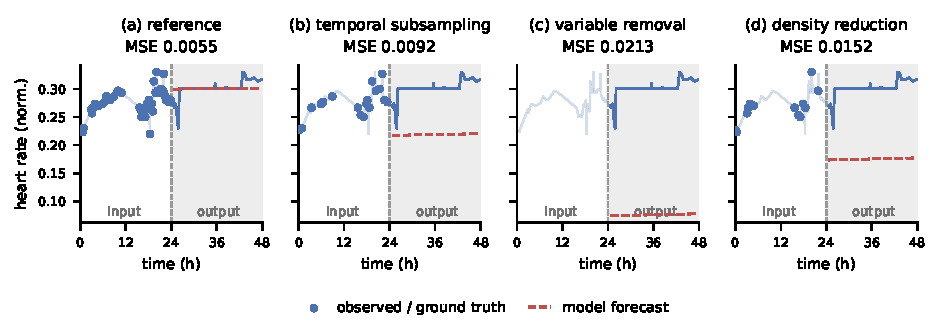
\includegraphics[width=\linewidth]{figures/fig2_observation_shift.pdf}
\caption{The same ICU history (heart rate and mean arterial pressure over 24\,h) observed through four
observation processes. The faint trajectory shows the underlying observations; markers indicate what the model
receives. The underlying history and the prediction target are identical across panels --- only the observation
process changes, moving one dimension of it at a time: how often measurements arrive (b), which variables are
recorded (c), and how many survive (d). The forecasting MSE of the same model under each condition is annotated
in each panel\prelim, so the change in predictive performance is attributable to the observation process alone.
Panels (b)--(d) are the evaluation conditions of Section~\ref{sec:splits}.}
\label{fig:views}
\end{figure}

The shift is easy to measure and can be large. Re-observing only the \emph{history} of each held-out input
through a different admissible process, with the prediction targets untouched (Figure~\ref{fig:views}), raises
the error of a wearable-sensor forecaster by a factor of nineteen and of a clinical forecaster by a factor of
two, while leaving a climate forecaster essentially unaffected. Two controlled comparisons sharpen this.
Observation density does not determine the damage: among processes that each delete about half of the
observations, error varies by up to $3.8\times$ depending on which half. And the damaging \emph{kind} of loss is
modality-dependent, with removal of whole variables dominating on clinical records and temporal subsampling
dominating on body-sensor records. A method that treats irregularity as a scalar corruption level cannot
represent either observation.

The starting point for our method is an asymmetry between training and deployment. At deployment the model is
given whatever the observation process supplies, and no more. During training, however, the same history can be
re-observed as often as we like, including through a process \emph{richer} than the one the model will face.
That richer observation is never available at test time, which makes it privileged information in the sense of
Learning Using Privileged Information \cite{vapnik2015lupi}: a training-time signal about the trajectory that the deployment view only partly
reveals.

We turn this into a training mechanism we call \emph{privileged observation self-distillation} (POSD). A teacher
$f_{\theta_T}$ receives a rich observation $\Sobs_{\mathrm{rich}}(X)$ of a history; a student $f_\theta$
receives a sparse observation $\Sobs(X)$ of the \emph{same} history, over the same prediction times and with the
same supervision; and the student is trained to match the teacher's task-level output in addition to the ground
truth. The teacher is not a larger or better-trained model, and it does not solve a different problem: it is the
same predictive model family with more information about the same trajectory. Its output therefore encodes what
is predictable from that trajectory when less of it has been discarded, which is exactly the target the student
should aim at from its restricted view. The teacher, the rich view and its extra forward pass all disappear
after training.

POSD is supported by a second mechanism and, conditionally, a third. \emph{Observation-process augmentation}
draws several observation processes per training trajectory from a mixture and trains on all of the resulting
views, treating the process as nuisance variation to randomise over; it is what exposes the student to process
variation in the first place, and it is the source of most of the robustness we measure. \emph{Hard
observation-process mining} instead searches a constrained candidate pool for the admissible process the current
model handles worst. Because its benefit turns on a property of the candidate pool rather than of the mechanism,
we keep it out of the headline configuration: 	extbf{OPERA} is augmentation plus privileged distillation, and
	extbf{OPERA++} adds mining from a pool strictly harsher than the training mixture.

Empirically, augmentation reduces relative degradation under shift from $+107\%$ to $+14\%$ on clinical
forecasting and from $+1793\%$ to $+25\%$ on wearable-sensor forecasting while leaving clean error unchanged, and
it transfers to observation-process \emph{families} that never appear in training. POSD adds a complementary
gain where augmentation alone does not help: on climate forecasting it improves clean error from $0.5329$ to
$0.5135$ and shifted error on every condition, and on sepsis prediction the complete configuration raises clean
AUROC from $82.1$ to $85.6$. Parameter count and inference latency are unchanged throughout.

\paragraph{Contributions.}
\begin{itemize}
\item \textbf{Observation-process shift.} We formalise observation-process shift as a distinct source of
distribution shift for irregular time series, give a composable removal-only family of observation processes
with validity constraints, and define a controlled protocol that re-observes held-out histories while preserving
targets, together with a train/test split over process families that makes generalisation measurable
(Sections~\ref{sec:problem} and \ref{sec:setup}).
\item \textbf{Privileged observation self-distillation.} We introduce a training mechanism in which a richer
observation of the same history supplies privileged task-level supervision to a student restricted to the
deployment observation, and we state and verify the invariant that separates it from label leakage: teacher and
student may differ only in the observation of the history (Section~\ref{sec:method}).
\item \textbf{Empirical robustness and its boundaries.} Across forecasting and classification benchmarks we show
that exposure to diverse observation processes substantially improves robustness, that privileged distillation
provides a complementary gain concentrated on information-limited tasks, and that hard mining helps only when its
candidate pool contains processes harsher than those augmentation already supplies (Section~\ref{sec:results}).
\end{itemize}

We use a query-based irregular encoder \cite{lim2026quite} as the experimental substrate because it consumes
irregular observations natively. Nothing in the formulation depends on that choice, and we report results on a
second backbone.

%% Related work, organised by scientific problem rather than by method lineage.
%% Included by sigconf.tex. Do not add a preamble here.

\section{Related Work}
\paragraph{Irregular multivariate time series.}
Interpolation-based methods map observations onto a regular grid before encoding \cite{shukla2019ipn};
continuous-time methods evolve a latent state between observations
\cite{rubanova2019latentode,debrouwer2019gruodebayes,kidger2020ncde}; set-based methods aggregate an unordered
observation set with attention \cite{horn2020seft,shukla2021mtand}; graph-based methods model inter-variable
structure \cite{zhang2022raindrop,zhang2024tpatchgnn}. Query-based embeddings \cite{lim2026quite} aggregate the
observations belonging to a variable or temporal patch into a fixed-size token, letting standard backbones
\cite{liu2024itransformer,nie2023patchtst} be reused unchanged. We do not propose a new encoder; we ask how any
such encoder behaves when the observation process moves.

\paragraph{Missingness mechanisms.}
The statistical literature classifies missingness by its dependence on observed and unobserved values
\cite{rubin1976missing}, and in clinical data the missingness pattern is itself informative
\cite{lipton2016informative,che2018grud}. Learning work typically treats irregularity as a property of a dataset
and probes robustness by varying a missingness \emph{rate}. We instead vary the observation \emph{process} at
comparable density and study the case where it differs between training and deployment.

\paragraph{Robustness through exposure and through constraint.}
Randomising nuisance factors during training is standard in sim-to-real transfer
\cite{tobin2017domainrand} and time-series augmentation \cite{wen2021augmentation}; invariant-risk formulations
instead constrain the representation across environments \cite{arjovsky2019irm}. Our observation views randomise
the measurement process rather than the signal. We deliberately do not impose cross-view representation
equality: objectives of that form are known to require explicit anti-collapse terms
\cite{chen2020simclr,grill2020byol,bardes2022vicreg}, and the property we need is that different observation
processes yield representations that remain \emph{useful}, not identical.

\paragraph{Privileged information and distillation.}
Learning with side information available only at training time is the LUPI setting \cite{vapnik2015lupi};
distillation \cite{hinton2015distilling} is one way to realise it, and the two are formally connected
\cite{lopezpaz2016unifying}. A richer observation of the same history is a natural privileged signal for
irregular data, which is the form we adopt.

\paragraph{Hard example and worst-case training.}
Selecting difficult examples accelerates and sharpens training \cite{shrivastava2016ohem}, and training against
a constrained worst case is the basis of adversarial robustness \cite{madry2018towards}. We apply the idea to
the observation process rather than to the input values, which keeps the perturbation set physically meaningful:
every candidate is a valid way the same trajectory could have been recorded.

%% Problem formulation, the three dimensions of an observation process, and the re-observation protocol.
%% Included by sigconf.tex. Do not add a preamble here.

\section{Observation-Process Shift}
\label{sec:problem}

\subsection{Problem formulation}
Let $X=\{x(t)\}_{t\in\mathcal{T}}$, $x(t)\in\mathbb{R}^{N}$, be an underlying multivariate temporal process over
a window $\mathcal{T}$. The learner never observes $X$. It receives a finite set of timestamped, partially
observed measurements
\begin{equation}
\Oobs=\{(t_k,\,x(t_k),\,m_k)\}_{k=1}^{K},\qquad m_k\in\{0,1\}^{N},
\end{equation}
where $m_{k,i}=1$ iff variable $i$ was measured at time $t_k$. The mechanism that selects $\{(t_k,m_k)\}$ is the
\emph{observation process} $\Sobs$; we write $\Oobs=\Sobs(X)$ and model it as a random variable
$\Sobs\sim P(\Sobs)$. A model $f_\theta$ maps $\Oobs$ to a task output $\hat Y$, either a forecast of $x$ over a
future window or a label.

Training and test data are drawn from joint distributions over $(X,\Sobs)$, and we separate two ways they can
differ:
\begin{equation}
P_{\mathrm{train}}(X)\ \neq\ P_{\mathrm{test}}(X)
\qquad\textit{(process shift)},
\end{equation}
\begin{equation}
P_{\mathrm{train}}(\Sobs)\ \neq\ P_{\mathrm{test}}(\Sobs)
\qquad\textit{(observation-process shift)}.
\end{equation}
This paper concerns the second, with $P(X)$ comparable. A protocol that draws training and test data from one
observation process cannot see it.

\subsection{Three dimensions of an observation process}
\label{sec:family}
An observation process is not a scalar. Because $\Sobs$ acts on a mask indexed by both time and variable, it can
differ from another process in three elementary ways: in \emph{how much} it records, in \emph{when} it records,
and in \emph{which variables} it records. We organise both the process family and the evaluation protocol around
those three dimensions, so that a measured degradation can be attributed to one of them.

We require the processes to be \emph{realisable}: each must correspond to a way the same trajectory could have
been recorded, so that the target stays well defined. We therefore admit only processes that act on the mask by
\emph{removal},
\begin{equation}
\Sobs:(t,m)\ \mapsto\ (t,\,m\odot\kappa),\qquad \kappa\in\{0,1\}^{K\times N},
\end{equation}
with values at removed entries discarded rather than imputed. Every $\Sobs(X)$ is then a sub-sample of the
original record and no artificial value is introduced, which is what permits one held-out set to be re-observed
many times with its supervision untouched.

Nine primitives instantiate the three dimensions:
\begin{itemize}
\item \textbf{density} --- how much survives. \textsc{RandomDropout}$(p)$ removes each observation independently
with probability $p$; \textsc{DensityControlledSampling}$(\rho)$ retains a fixed fraction $\rho$ of every
variable's observations, fixing density independently of the original pattern.
\item \textbf{timing} --- when observations arrive. \textsc{TemporalStride}$(k)$ keeps every $k$-th observation
of each variable, lowering the sampling \emph{rate} while keeping it regular; \textsc{BurstMissingness}$(p)$
removes contiguous windows covering a fraction $p$ of the observed span; \textsc{LongGapMissingness}$(p)$ is the
single-window case; \textsc{LocalTemporalMask}$(p)$ removes one contiguous run per variable, matching random
dropout in density but clustering the loss within each channel.
\item \textbf{variable availability} --- which channels exist at all. \textsc{VariableDropout}$(p)$ removes whole
variables independently; \textsc{VariableGroupDropout}$(p)$ removes contiguous blocks of variables together,
modelling a failed monitor or an unavailable panel.
\end{itemize}
Processes compose sequentially ($\Sobs_2\circ\Sobs_1$, written \texttt{a+b}) and mix
($\Sobs\sim\mathrm{Unif}\{\Sobs_1,\dots\}$, written \texttt{a|b}), so an observation regime is specified by a
string rather than by code, and a process can move two dimensions at once.

\paragraph{The dimensions are not separable at the level of a single variable.}
It is tempting to summarise what a process did to variable $i$ by how many of its observations survived, and to
expect the error on variable $i$ to follow. It does not, because $f_\theta$ predicts each variable from the whole
observation. Two processes can leave one channel exactly the same observations and still produce very different
error on it, if they differ in what they removed from the \emph{other} channels
(Figure~\ref{fig:views}). A per-variable missingness rate is therefore not a sufficient statistic for the damage,
which is the concrete sense in which the observation process has to be treated as a structured object.

\subsection{Controlled re-observation and validity}
\label{sec:reobs}
Observation-process shift is measured by re-observation. For an evaluation process $\Sobs$ we replace the
\emph{history} of each held-out input by $\Sobs$ applied to it, and leave the prediction times, forecast targets
and labels exactly as they were. The comparison therefore isolates the observation process: the underlying
trajectory and the supervision are held fixed by construction, and a single test set yields as many shifted
conditions as there are processes. The pseudo-random draw is seeded independently of the run, so every model is
scored on byte-identical re-observed inputs and comparisons are paired at the level of individual test inputs.
The \emph{clean} condition is the dataset's own observation process, $\Sobs=\mathrm{id}$.

Because two of our mechanisms select observation processes rather than merely sampling them, we also need to rule
out degenerate choices. We impose validity constraints $\mathcal{C}$ on relative density, variable coverage,
maximum gap and observation count,
\begin{equation}
\mathcal{C}:\quad \rho_{\min}\le\frac{\rho(\Sobs(X))}{\rho(X)}\le\rho_{\max},\quad
\Delta t_{\max}(\Sobs(X))\le G_{\max},\quad \dots
\label{eq:constraints}
\end{equation}
and discard any candidate that violates a bound before it can be selected. Throughout we use
$\rho_{\min}=0.15$, variable coverage $\ge0.3$, $G_{\max}=0.6$ of the window and at least four observations per
sample. We additionally record a per-sample descriptor $r=g(\Oobs)\in\mathbb{R}^{8}$ of the realised process
(observation count and density, the mean, standard deviation and maximum inter-observation gap, temporal
coverage, variable coverage and recent density), computed from timestamps and masks alone and never from values,
which we use to report what a condition actually did to a batch.

%% Method. POSD is the centrepiece; augmentation supplies its views. OPERA = the two. OPERA++ = plus harsh-pool
%% mining, reported as a variant. Mining over the training mixture is a control, never an arm.
%% Included by sigconf.tex. Do not add a preamble here.

\section{Privileged Observation Self-Distillation}
\label{sec:method}

\begin{figure}[t]
\centering
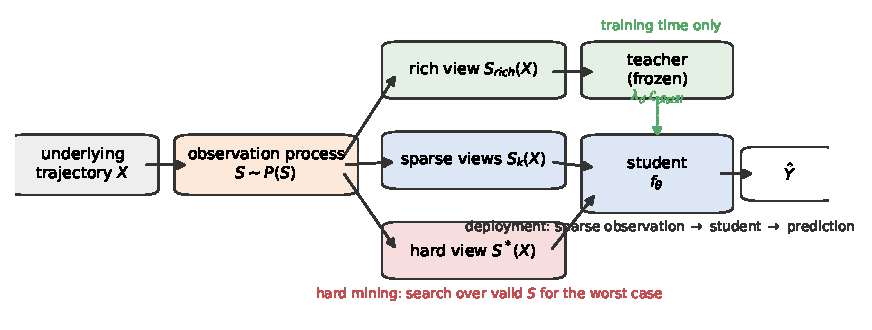
\includegraphics[width=\linewidth]{figures/fig1_framework.pdf}
\caption{The student is restricted to a sparse observation of a trajectory; the teacher receives a richer
observation of the \emph{same history}, over the same prediction times and with the same supervision, and its
task output becomes an additional target for the student (dashed). Observation-process augmentation supplies the
student's views. OPERA is these two mechanisms; OPERA++ additionally replaces some views with the hardest
candidate from a pool harsher than the training mixture. At deployment only the student and one sparse
observation remain.}
\label{fig:framework}
\end{figure}

Everything in this section acts on $\Sobs$ rather than on the encoder: the architecture, its parameter count and
its inference path are untouched (Figure~\ref{fig:framework}). Two configurations are reported, and the
distinction matters because one mechanism turns out to be conditional on a hyper-parameter rather than
universally useful:
\begin{itemize}
\item \textbf{OPERA} $=$ privileged observation self-distillation $+$ observation-process augmentation. This is
the method: two mechanisms, no candidate pool to choose.
\item \textbf{OPERA++} $=$ OPERA $+$ hard observation-process mining from a pool strictly harsher than the
training mixture. It buys worst-case robustness for $K$ extra forward passes per step and one more
hyper-parameter.
\end{itemize}
Mining over the training mixture itself is neither configuration. It is the control that establishes why pool
severity matters, and we report it as an ablation (Section~\ref{sec:mining-results}). We introduce distillation
first, as the mechanism we regard as the contribution, then the augmentation that feeds it, then the objective
that defines OPERA, and finally the mining variant.

\subsection{Rich and sparse observations of one history}
\label{sec:distill}
At deployment a model receives whatever its observation process supplies. During training the same history can be
re-observed at will, and in particular it can be observed \emph{more richly} than deployment permits. Write
\begin{equation}
\Oobs_s=\Sobs_s(X),\qquad \Oobs_r=\Sobs_r(X),
\label{eq:richsparse}
\end{equation}
where $\Sobs_s$ is a deployment-constrained observation process and $\Sobs_r$ is at least as dense as $\Sobs_s$ on
the same trajectory; in our experiments $\Sobs_r$ is the untouched record. Because $\Oobs_r$ exists only at
training time it is privileged information in the sense of \cite{vapnik2015lupi}, and distillation
\cite{hinton2015distilling,lopezpaz2016unifying} is the natural way to route it into the student.

\subsection{The distillation objective}
A teacher $f_{\theta_T}$ is trained on rich observations and then frozen. The student $f_\theta$ is trained on
sparse observations of the same histories and, in addition to the task loss, is asked to reproduce the teacher's
task-level output:
\begin{equation}
\hat Y_T=f_{\theta_T}(\Oobs_r),\qquad \hat Y_S=f_\theta(\Oobs_s),
\label{eq:studteach}
\end{equation}
\begin{equation}
\mathcal{L}_{\mathrm{distill}}=D\big(\hat Y_S,\ \mathrm{sg}[\hat Y_T]\big)
=\big\|\hat Y_S-\mathrm{sg}[\hat Y_T]\big\|^{2}_{\Omega},
\label{eq:distill}
\end{equation}
where $\mathrm{sg}[\cdot]$ is the stop-gradient and $\Omega$ restricts the norm to entries that carry supervision,
so the student is never asked to imitate the teacher where no target exists. For probabilistic outputs $D$ may
instead be a KL divergence. We also implement an exponential-moving-average teacher,
$\theta_T\leftarrow\alpha_T\theta_T+(1-\alpha_T)\theta$, and treat frozen-versus-EMA as an empirical choice; the
reported runs use a frozen teacher.

The value of this term is not that the teacher is a better model. Teacher and student share capacity, family and
objective, and the teacher is ahead only because less of the trajectory was discarded before it saw it. Its output
describes what is predictable from that trajectory under a smaller observation loss, and the student is pushed
toward that value from a view in which part of the same structure has been removed. Stated precisely, the teacher
exposes the student to prediction-relevant information that is present in the underlying history but partially
obscured by the deployment observation process. It does not tell the student which observations will be available:
that is fixed by the deployment process and is not something the student can act on.

\paragraph{Why the teacher has something to offer.}
Section~\ref{sec:family} noted that a variable is predicted from the whole observation, not from its own channel,
so removing one channel degrades the others. The converse is what makes the rich view informative: an observation
that retains channels the student's view lost supports a prediction the student cannot reconstruct from what it
holds. The teacher's output is a summary of that, at exactly the granularity the task is scored on.

\paragraph{Why this is self-distillation.}
The asymmetry between the two networks lies entirely in the observation. The teacher is not a separately designed
expert, a larger network, or a model solving a different task; it is the same predictive model family evaluated on
a richer view of the same sample. Teacher--student distillation is not new and we do not claim it is. What is
specific here is the \emph{source and structure of the privileged signal}: it is produced by choosing a different
observation process for a history the student already holds, which requires no extra annotation, no extra sensor
and no extra data. In our experiments it also requires no extra training run, because the teacher is the
unmodified baseline for the same setting, backbone and seed.

\paragraph{The anti-leakage invariant.}
Teacher and student must differ \emph{only} in the observation of the history. Both are evaluated over the same
history window, the same prediction times and the same supervision, so the teacher never sees a future value or a
label that the student is denied. Without this restriction the term would degenerate into label leakage and any
apparent gain would be uninterpretable. We enforce it with an assertion over every batch key that carries
supervision, for both forecasting and classification, and test it directly.

\paragraph{At inference.}
The student consumes one sparse observation and emits a prediction. The teacher, the rich view and the extra
forward pass are training-time constructs; the student never receives a rich observation at test time.

\subsection{Observation-process augmentation}
\label{sec:aug}
Privileged distillation needs the student to be trained on sparse views, and the views it trains on determine what
it has to recover. The supporting mechanism supplies them by treating the observation process as nuisance
variation to randomise over: for each training trajectory we draw $V$ processes from a mixture $P_{\mathrm{mix}}$
and train on every resulting view,
\begin{equation}
\Oobs_v=\Sobs_v(X),\quad \Sobs_v\sim P_{\mathrm{mix}},\qquad
\mathcal{L}_{\mathrm{task}}=\frac1V\sum_{v=1}^{V}\ell\big(f_\theta(\Oobs_v),\,Y\big),
\label{eq:aug}
\end{equation}
with $\ell$ the masked mean squared error for forecasting and cross-entropy for classification. The targets $Y$
are shared across views and never modified: every view is a different recording of the same episode. The mixture
spans all three dimensions of Section~\ref{sec:family}, since exposure to one of them does not confer robustness
to the others.

We impose no representation-level requirement. The property we want is that $f_\theta(\Sobs_1(X))$ and
$f_\theta(\Sobs_2(X))$ both remain useful for the task, which is weaker than requiring the latent codes
$z(\Sobs_1(X))$ and $z(\Sobs_2(X))$ to agree. The weaker property is the safer one: a representation-matching
penalty admits the degenerate solution of collapsing all observations of all trajectories together, and preventing
that needs anti-collapse machinery unrelated to the shift under study. A representation-matching variant exists in
our implementation and is reported only as an ablation.

\subsection{The objective, and what OPERA is}
OPERA adds one term to the task loss,
\begin{equation}
\fbox{$\displaystyle\ \mathcal{L}=\mathcal{L}_{\mathrm{task}}+\lambda_{d}\,\mathcal{L}_{\mathrm{distill}}\ $}
\label{eq:objective}
\end{equation}
with $\mathcal{L}_{\mathrm{task}}$ from Eq.~\ref{eq:aug} over $V$ augmented views and
$\mathcal{L}_{\mathrm{distill}}$ from Eq.~\ref{eq:distill} against the frozen rich-view teacher. No other loss is
introduced, and in particular no representation-consistency term. Setting $\lambda_d=0$ and $V=1$ recovers
ordinary training. We use $\lambda_d=1$, $V=2$ and a frozen teacher throughout. Algorithm~\ref{alg:opera} is a
single update: one loss, one backward pass, one optimiser step, and the only staging is that the teacher is
trained beforehand --- which in our setup costs nothing extra, since it is the baseline run for that cell.

\begin{algorithm}[t]
\caption{One OPERA training step (OPERA++ adds the bracketed branch)}
\label{alg:opera}
\begin{algorithmic}[1]
\Require batch $(X,Y)$ with observation $(t,m)$; mixture $P_{\mathrm{mix}}$; frozen teacher $f_{\theta_T}$;
\emph{for OPERA++:} epoch $e$, pool $\mathcal{P}$, constraints $\mathcal{C}$, ratio $\alpha$
\State $\{\Sobs_v\}_{v=1}^{V}\sim P_{\mathrm{mix}}$
\If{OPERA++ \textbf{and} $e\ge e_{\mathrm{warm}}$}
  \State draw $K$ candidates from $\mathcal{P}$; keep those satisfying $\mathcal{C}$
  \State score survivors with $f_\theta$ under \texttt{no\_grad}; replace $\lceil\alpha V\rceil$ views with the hardest
\EndIf
\State $\hat{Y}_T \gets \mathrm{sg}\big[f_{\theta_T}(\Sobs_{r}(X))\big]$ \Comment{same history, richer view}
\State $\mathcal{L}\gets\frac1V\sum_v \ell(f_\theta(\Sobs_v(X)),Y) + \lambda_d\sum_v \mathcal{L}_{\mathrm{distill}}$
\State one optimiser step on $\mathcal{L}$
\end{algorithmic}
\end{algorithm}

\subsection{OPERA++: hard observation-process mining}
\label{sec:mining}
Random exposure spends most of its budget on observation processes the model already handles. The variant searches
instead for the admissible process the \emph{current} model handles worst,
\begin{equation}
\Sobs^{*}=\arg\max_{\Sobs\in\mathcal{A}}\ \ell\big(f_\theta(\Sobs(X)),Y\big),
\qquad \mathcal{A}=\{\Sobs:\ \Sobs\ \mathrm{satisfies}\ \mathcal{C}\},
\label{eq:mining}
\end{equation}
with $\mathcal{C}$ from Eq.~\ref{eq:constraints}. We do not differentiate through mask generation. We approximate
the maximisation by scoring a finite candidate pool: $K$ candidates are drawn from a pool $\mathcal{P}$, filtered
through $\mathcal{C}$, scored under \texttt{no\_grad}, and the hardest survivors retained. Only selected views
enter the backward pass, so mining costs $K$ extra forward passes and no extra gradient memory. We call this hard
observation-process mining, or approximate worst-case observation-process selection, rather than adversarial
training: the maximisation runs over a discrete pool of physically valid recordings rather than a norm ball, and it
is neither exact nor differentiable.

Training only on hard views destabilises optimisation and biases the student away from the deployment regime, so
we mix,
\begin{equation}
P(\Sobs)=(1-\alpha)\,P_{\mathrm{mix}}+\alpha\,P_{\mathrm{hard}},
\label{eq:alpha}
\end{equation}
and hold $\alpha=0$ during a warm-up period; we use $K=4$ and $\alpha=0.5$ after five epochs. The consequential
choice is $\mathcal{P}$. If $\mathcal{P}=P_{\mathrm{mix}}$ then the hardest of $K$ draws is close in severity to a
single draw and the mechanism reduces to augmentation at $K$ times the cost. OPERA++ is therefore \emph{defined}
by a pool strictly harsher than $P_{\mathrm{mix}}$, and the matched-pool setting is reported only as the control
that establishes the distinction (Section~\ref{sec:mining-results}).

%% Experimental setup: datasets, the disjoint observation-process splits, metrics, protocol.
%% Included by sigconf.tex. Do not add a preamble here.

\section{Experimental Setup}
\label{sec:setup}

\subsection{Datasets and tasks}
We use five datasets spanning three sensing modalities, two tasks and two backbones
(Table~\ref{tab:datasets}). Preprocessing, splits and normalisation are the unmodified published pipelines:
t-PatchGNN \cite{zhang2024tpatchgnn} for the forecasting benchmarks (PhysioNet from the 2012 challenge
\cite{silva2012physionet}) and Raindrop \cite{zhang2022raindrop} for classification, including the
minority-class upsampling of the binary tasks. USHCN appears at two horizons because horizon length changes how
much a model must rely on its history, which turns out to change its sensitivity to the shift.

\begin{table}[t]
\caption{Datasets and task settings. Backbone follows the published protocol per task.}
\label{tab:datasets}
\small
\begin{tabular}{llrrll}
\toprule
setting & task & vars & samples & backbone & metric \\
\midrule
PhysioNet 24h$\to$24h & forecast & 41 & 12{,}000 & iTransformer & MSE \\
Activity 3000$\to$1000\,ms & forecast & 12 & 5{,}400 & iTransformer & MSE \\
USHCN 24$\to$1 mo & forecast & 5 & 26{,}736 & iTransformer & MSE \\
USHCN 24$\to$12 mo & forecast & 5 & 26{,}736 & iTransformer & MSE \\
P12 mortality & classify (2) & 36 & 11{,}988 & PatchTST & AUROC \\
P19 sepsis & classify (2) & 34 & 38{,}803 & PatchTST & AUROC \\
PAM activity & classify (8) & 17 & 5{,}333 & PatchTST & accuracy \\
\bottomrule
\end{tabular}
\end{table}

\subsection{Observation-process splits}
\label{sec:splits}
Training and evaluation draw from \emph{disjoint} observation-process distributions, so that generalisation across
observation processes is measured rather than assumed.

\textbf{Training pool} $P_{\mathrm{mix}}$ is deliberately mild: random dropout at $p\in\{0.1,0.25,0.4\}$, stride
$2$, burst at $p\in\{0.2,0.3\}$, variable dropout at $p=0.2$ and local masking at $p=0.3$.

\textbf{Evaluation conditions} are the clean condition plus 15 shifted processes, each applied by the
re-observation protocol of Section~\ref{sec:reobs}. Nine are designated \emph{unseen} because their family never
appears in the training pool: random dropout $0.7$, variable dropout $0.5$, stride $3$ and $4$, long gap $0.4$,
burst $0.5$, variable-group dropout $0.3$, and two compositions (random $0.5$ $+$ variable $0.3$; stride $3$ $+$
variable-group $0.3$). The remaining six re-use training families at severities outside the pool, together with
density-controlled sampling at $\rho=0.5$. We report degradation over all fifteen shifted conditions and,
separately, over the nine unseen ones.

\textbf{Mining candidate pool.} Two pool constructions are reported. $\mathcal{P}=P_{\mathrm{mix}}$ is the natural
default: mining over the processes the model already trains on. The \emph{harsher} pool adds severities and
pairwise compositions beyond $P_{\mathrm{mix}}$ while remaining disjoint from the evaluation conditions, so no
evaluation process is ever mined.

\subsection{Metrics}
Forecasting uses masked MSE and MAE over observed target entries, averaged per variable and then over variables
with supervision. Binary classification uses AUROC and AUPRC; the eight-class task uses accuracy and macro F1. We
summarise sensitivity by the relative degradation of a model with respect to its \emph{own} clean score,
\begin{equation}
\Delta_{\mathrm{shift}}=\frac{1}{|\mathcal{E}|}\sum_{\Sobs\in\mathcal{E}}
\frac{\mathrm{err}_{\Sobs}-\mathrm{err}_{\mathrm{clean}}}{\mathrm{err}_{\mathrm{clean}}},
\label{eq:degradation}
\end{equation}
over the shifted conditions $\mathcal{E}$, and report the same quantity restricted to the unseen subset. For
classification we take $\mathrm{err}=1-\mathrm{AUROC}$ (or $1-\mathrm{accuracy}$) so that $\Delta$ is computed on
the same metric used to judge the task; cross-entropy degradation can move in the opposite direction to AUROC and
we do not use it as a headline number.

Two cautions govern how we read Eq.~\ref{eq:degradation}. It is normalised by a model's own clean score, so a
uniformly weaker model can post a flattering ratio, and it says nothing about attainable error. We therefore report
clean, mean shifted and worst-case absolute performance in every table and treat $\Delta_{\mathrm{shift}}$ as a
secondary summary that must be read beside them. We also report parameter count, training time per epoch, peak
training memory and inference latency.

\subsection{Protocol}
All models use the query-based irregular embedding with hidden width 64, four heads and three layers, trained with
Adam at $10^{-3}$, batch 32 (128 for USHCN; 16 for P12, where a single view's attention already occupies
4.7\,GB), an epoch cap of 40, early-stopping patience 10 and a minimum of 15 epochs. Configurations that are
compared are trained at identical batch size. Runs execute sequentially on one 8\,GB GPU, and every run records
its configuration, git commit, seed, checkpoint and metrics. \textbf{All reported numbers use a single seed} and
are marked \prelim; the protocol calls for five paired seeds, and we regard nothing reported here as a statistical
result. \todo{five paired seeds for the primary comparisons}

%% Establishing the phenomenon on models trained without any OPERA mechanism (Tables 2-3).
%% Included by sigconf.tex. Do not add a preamble here.

\section{Does Observation-Process Shift Matter?}
\label{sec:phenomenon}
We first establish the phenomenon on models trained without any OPERA mechanism.

\paragraph{Severity spans three orders of magnitude.}
Table~\ref{tab:phenomenon} reports each baseline under its own observation process and under shift. Mean
degradation ranges from $+1.9\%$ to $+1793\%$, and the ordering is interpretable: it grows with how much of the
task's predictive signal must come from the irregular history. USHCN forecasting one month ahead from five
climate variables sits at the bottom, and the diagnostic is unambiguous --- removing half of its observations at
matched density \emph{lowers} its error, from $0.5379$ to $0.5355$. Its signal is carried by seasonal structure
that survives the loss. Extending the same dataset to a twelve-month horizon doubles its sensitivity
($+1.9\%\to+3.7\%$), which identifies the mechanism of the null rather than excusing it. At the top, Activity's
millisecond-resolution sensor dynamics degrade by $32\times$ under stride-4 subsampling alone.

\begin{table}[t]
\caption{Observation-process shift on models trained without any OPERA mechanism\prelim. Primary metric per
setting; degradation by Eq.~\ref{eq:degradation}. Every shifted condition re-observes only the history.}
\label{tab:phenomenon}
\small
\begin{tabular}{lrrrr}
\toprule
setting & clean & worst condition & $\Delta_{\mathrm{shift}}$ & $\Delta_{\mathrm{unseen}}$ \\
\midrule
Activity (MSE) & 0.00263 & 0.08547 \textit{(stride 4)} & $+1793\%$ & $+2057\%$ \\
PhysioNet (MSE) & 0.00549 & 0.02134 \textit{(var .5)} & $+107\%$ & $+130\%$ \\
PAM (acc.) & 88.01 & 53.93 \textit{(var .5)} & $+64\%$ & $+88\%$ \\
USHCN-12mo (MSE) & 0.52020 & 0.55338 \textit{(comp.)} & $+3.7\%$ & $+4.6\%$ \\
P19 (AUROC) & 82.13 & 74.63 \textit{(var .3)} & $+2.9\%$ & $+3.3\%$ \\
USHCN-1mo (MSE) & 0.53787 & 0.56933 \textit{(var .5)} & $+1.9\%$ & $+2.8\%$ \\
P12 (AUROC) & 83.53 & 77.98 \textit{(comp.)} & \multicolumn{2}{c}{\textit{see \S\ref{sec:analysis}}} \\
\bottomrule
\end{tabular}
\end{table}

\paragraph{Density does not explain it.}
Table~\ref{tab:density} compares processes that remove approximately half of the observations but destroy
different structure. On PhysioNet the spread is $2.9\times$ and on PAM $3.5\times$ in cross-entropy; a model can
lose half its observations almost for free if they are removed uniformly in time, and catastrophically if they
are removed by variable. Treating irregularity as a scalar corruption level cannot represent this distinction,
which is the empirical case for modelling the observation process as an object.

\begin{table}[t]
\caption{Matched-density comparison\prelim: four processes each removing $\approx$50\% of observations, on
models trained without OPERA. Error varies by $2.9$--$3.5\times$ with \emph{what} is removed.}
\label{tab:density}
\small
\begin{tabular}{lrrrr}
\toprule
 & density- & stride & burst & variable \\
setting & matched & 2 & .5 & dropout .5 \\
\midrule
PhysioNet (MSE) & 0.00736 & 0.00791 & 0.00804 & \textbf{0.02134} \\
Activity (MSE) & 0.04892 & 0.05230 & \textbf{0.01973} & 0.05778 \\
PAM (cross-ent.) & 0.4466 & 0.4360 & 0.4897 & \textbf{1.5578} \\
\bottomrule
\end{tabular}
\end{table}

\paragraph{The damaging kind of loss is modality-dependent.}
On the clinical datasets, losing whole variables dominates while temporal subsampling is nearly free: on P19,
removing 30\% of variables costs 7.5 AUROC whereas stride 3 costs 1.1; on PAM, removing half the variables costs
34 accuracy points whereas stride 3 costs 1.5. Activity inverts this, with stride its single worst condition and
burst removal its mildest (Table~\ref{tab:density}). Hourly laboratory values are largely redundant in time and
irreplaceable across channels; body-sensor dynamics are the reverse. A robustness method must therefore cover
process \emph{families}, not a severity axis.

%% Main results: mechanism isolation, cross-setting comparison, cost (Tables 4-6).
%% Included by sigconf.tex. Do not add a preamble here.

\section{Results}
\label{sec:results}

\begin{figure}[t]
\centering
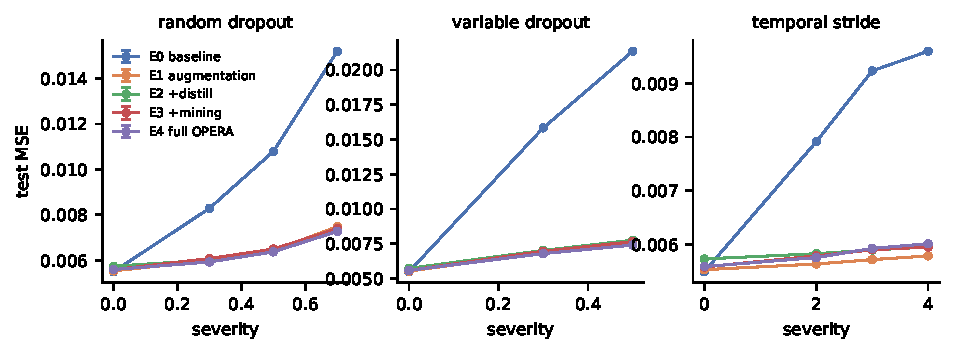
\includegraphics[width=\linewidth]{figures/fig3_robustness_curve.pdf}
\caption{Error against observation-process severity on PhysioNet\prelim, for three process families. Severity
$0$ is the dataset's own observation process. Without any mechanism (blue) error grows steeply in every family;
every OPERA configuration stays close to its clean error, including for stride subsampling, a family absent
from the training pool.}
\label{fig:curve}
\end{figure}

\paragraph{Exposure to diverse observation processes accounts for most of the attainable robustness.}
Table~\ref{tab:components} and Figure~\ref{fig:curve} isolate the mechanisms on PhysioNet. Augmentation alone
reduces $\Delta_{\mathrm{shift}}$ from $+107\%$ to $+14\%$ and $\Delta_{\mathrm{unseen}}$ from $+130\%$ to $+18\%$ while
leaving clean error unchanged ($0.00553$ vs.\ $0.00549$), and it improves all sixteen conditions. It transfers to
process families absent from training: stride subsampling, never trained on in any form, falls from $0.00923$ to
$0.00572$. On Activity the same mechanism, combined with the others, reduces mean shifted error from $0.04983$ to
$0.00358$, a factor of fourteen (Table~\ref{tab:main}).

\begin{table}[t]
\caption{Mechanism isolation on PhysioNet (test MSE\prelim). ``pool'' is the hard-mining candidate pool of
Section~\ref{sec:mining}. Read $\Delta$ beside the absolute columns.}
\label{tab:components}
\small
\begin{tabular}{lrrrr}
\toprule
configuration & clean & mean shift & worst & $\Delta_{\mathrm{shift}}$ \\
\midrule
no mechanism & \textbf{0.00549} & 0.01137 & 0.02134 & $+107.0\%$ \\
augmentation & 0.00553 & 0.00632 & 0.00772 & $+14.3\%$ \\
\quad $+$ distillation & 0.00573 & 0.00644 & 0.00776 & $+12.3\%$ \\
\quad $+$ mining, pool $=P_{\mathrm{mix}}$ & 0.00558 & 0.00641 & 0.00765 & $+14.8\%$ \\
\quad $+$ mining, harsher pool & 0.00562 & \textbf{0.00626} & \textbf{0.00721} & $+11.4\%$ \\
all three, pool $=P_{\mathrm{mix}}$ & 0.00559 & 0.00632 & 0.00741 & $+13.1\%$ \\
all three, harsher pool & 0.00590 & 0.00653 & 0.00748 & $\mathbf{+10.7\%}$ \\
\bottomrule
\end{tabular}
\end{table}

\paragraph{Adversarial selection of observation processes helps only when its candidates exceed the training
pool.} With $\mathcal{P}=P_{\mathrm{mix}}$, mining is indistinguishable from augmentation ($+14.8\%$ vs.\
$+14.3\%$; mean shifted $0.00641$ vs.\ $0.00632$) at $2.7\times$ the training cost, because the hardest of $K$
draws from the training mixture is barely harder than one draw. Given a pool containing severities and
compositions absent from training, the same mechanism becomes the strongest single configuration on absolute
shifted error and worst case ($0.00626$ and $0.00721$), with the gain concentrated exactly where it should be:
$0.00706$ vs.\ $0.00747$ under 70\% dropout and $0.00721$ vs.\ $0.00753$ under 50\% variable removal. This is a
property of the pool, not of the mechanism, and it is easy to miss: the natural default --- mining over the
processes one already trains on --- yields a null result.

\paragraph{Privileged distillation improves accuracy where the task is noisy, not robustness.}
On PhysioNet it is within noise of augmentation. On USHCN, where the task is hard and the student underfits, it
is the largest single effect we measure: clean MSE $0.5379\to0.5135$ ($-4.5\%$), best on thirteen of sixteen
conditions, while $\Delta_{\mathrm{shift}}$ does not improve. On P19 the full framework lifts clean AUROC
$82.13\to85.59$ and AUPRC $16.89\to24.47$ ($+45\%$). The pattern is consistent with distillation acting as a
smoother regression target rather than as a robustness mechanism.

\begin{figure}[t]
\centering
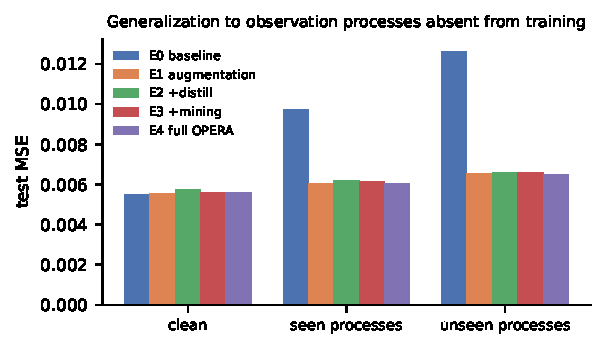
\includegraphics[width=0.85\linewidth]{figures/fig4_unseen_generalization.pdf}
\caption{Generalisation across the observation-process split on PhysioNet\prelim. ``Seen'' averages families
present in the training pool at unseen severities; ``unseen'' averages the nine conditions whose families never
appear in training (Section~\ref{sec:splits}). The gap between the two bars is small for every OPERA
configuration and large without any mechanism.}
\label{fig:unseen}
\end{figure}

\paragraph{Robustness extends to unseen process families.}
Figure~\ref{fig:unseen} separates conditions whose families appear in the training pool from those whose do
not. Without a mechanism the unseen group is worse than the seen group ($0.01260$ vs.\ $0.00975$) and both are
far above clean; with augmentation the three bars are nearly level ($0.00553$, $0.00604$, $0.00652$). The
mechanism therefore generalises across the split defined in Section~\ref{sec:splits} rather than memorising the
training pool.

\paragraph{Across settings, benefit tracks baseline damage.}
Table~\ref{tab:main} compares no mechanism against the full framework on every setting. Where degradation is
large the gains are large; where the baseline is already insensitive there is little to recover, and the
framework neither helps nor harms materially. On the classification tasks the effect appears in the primary
metric: PAM recovers $10.5$ and $11.1$ accuracy points at 30\% and 50\% variable removal, P19 gains $5.6$ AUROC
at 30\% variable removal and improves clean accuracy as well, and P12 --- which barely degrades --- gains $2.6$
AUROC at 50\% variable removal for a $0.2$ AUROC clean cost.

\begin{table}[t]
\caption{No mechanism vs.\ the full framework across all settings\prelim. Primary metric; MSE lower-better,
AUROC/accuracy higher-better. $\Delta$ is Eq.~\ref{eq:degradation} on the primary error.}
\label{tab:main}
\small
\begin{tabular}{llrrrr}
\toprule
 &  & \multicolumn{2}{c}{no mechanism} & \multicolumn{2}{c}{full OPERA} \\
\cmidrule(lr){3-4}\cmidrule(lr){5-6}
setting & metric & clean & $\Delta$ & clean & $\Delta$ \\
\midrule
Activity & MSE & \textbf{0.00263} & $+1793\%$ & 0.00286 & $\mathbf{+25\%}$ \\
PhysioNet & MSE & \textbf{0.00549} & $+107\%$ & 0.00559 & $\mathbf{+13\%}$ \\
PAM & acc. & \textbf{88.01} & $+64\%$ & 87.27 & $\mathbf{+34\%}$ \\
USHCN-12mo & MSE & 0.52020 & $+3.7\%$ & \textbf{0.51686} & $\mathbf{+2.6\%}$ \\
P19 & AUROC & 82.13 & $+2.9\%$ & \textbf{85.59} & $\mathbf{+1.2\%}$ \\
USHCN-1mo & MSE & 0.53787 & $+1.9\%$ & \textbf{0.52107} & $\mathbf{+1.5\%}$ \\
P12 & AUROC & \textbf{83.53} & --- & 83.30 & --- \\
\bottomrule
\end{tabular}
\end{table}

\begin{figure}[t]
\centering
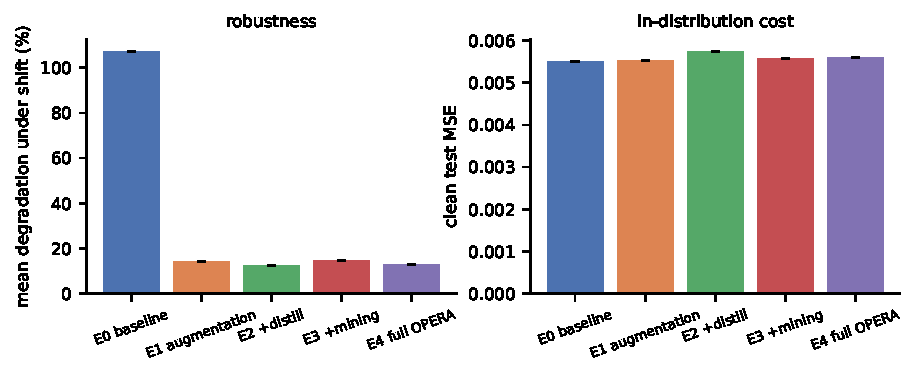
\includegraphics[width=\linewidth]{figures/fig5_ablation.pdf}
\caption{Contribution of each mechanism on PhysioNet\prelim: mean degradation under shift (left, lower is
better) against in-distribution error (right). Robustness improves by roughly an order of magnitude while
clean error moves within $0.0004$\,MSE, so the mechanisms are not trading in-distribution accuracy for
robustness.}
\label{fig:ablation}
\end{figure}

\paragraph{Cost.}
Figure~\ref{fig:ablation} summarises the trade and Table~\ref{tab:cost} the overhead. Every mechanism is
training-time only: parameter count is identical
across configurations and inference latency is unchanged at $0.63$\,ms per series. Augmentation costs
$1.7\times$ time and $1.7\times$ peak memory for two views; mining adds $K$ forward passes per step.

\begin{table}[t]
\caption{Training and deployment cost on PhysioNet\prelim. Inference and parameter count are unaffected by
every mechanism.}
\label{tab:cost}
\small
\begin{tabular}{lrrrr}
\toprule
configuration & params & s/epoch & peak GB & infer.\ ms \\
\midrule
no mechanism & 129{,}153 & 24.1 & 3.7 & 0.630 \\
augmentation & 129{,}153 & 41.4 & 6.3 & 0.670 \\
$+$ distillation & 129{,}153 & 45.3 & 6.3 & 0.630 \\
$+$ mining (harsher pool) & 129{,}153 & 82.3 & 6.3 & 0.634 \\
all three (harsher pool) & 129{,}153 & 86.3 & 6.3 & 0.629 \\
\bottomrule
\end{tabular}
\end{table}

%% Analysis of the negative/partial results, the degradation-ratio pitfall, and limitations.
%% Included by sigconf.tex. Do not add a preamble here.

\section{Analysis and Limitations}
\label{sec:analysis}

\paragraph{What the negative and partial results delimit.}
Two mechanisms did not behave as their motivation suggested, and both boundaries are informative. Mining's
inertness under its natural default shows that "train on the worst case" is empty unless the search space
exceeds what random exposure already covers. Distillation's profile shows that a richer observation helps when
the student cannot fit the target, which is a statement about task noise rather than about observation-process
shift; the two goals are separable and should not be conflated because both happen to involve sparse views.
Conversely, augmentation's dominance is itself a finding: informing a model by \emph{showing} it varied
observation processes was consistently more reliable than constraining what its representation must look like.

\paragraph{When the ratio metric misleads.}
P12's cross-entropy \emph{improves} under mild shifts while its AUROC and AUPRC fall, so
$\Delta_{\mathrm{shift}}$ computed on cross-entropy is negative and meaningless there; we omit it in
Table~\ref{tab:main} and read P12 from the ranking metrics. More generally, because
Eq.~\ref{eq:degradation} normalises by a model's own clean score, a uniformly weaker model can post a better
ratio. On USHCN-1mo the baseline's ratio ($+1.9\%$) is close to the framework's ($+1.5\%$) while its shifted
error is higher everywhere, and its clean error exceeds the framework's error \emph{under shift}. Absolute
error remains the quantity of interest. \todo{recompute degradation on AUROC for binary tasks}

\paragraph{Limitations.}
Every number is single-seed; the protocol requires five, and the smaller differences in
Tables~\ref{tab:components} and \ref{tab:main} are within the range we would expect seeds to move. Observation
processes are synthetic re-observations of real records, which is what makes the targets well defined but is
weaker evidence than a shift between two real acquisition environments. Compositions are limited to pairs. The
two backbones are tied to tasks rather than crossed with them. USHCN is not min-max normalised by its published
pipeline, so its errors are in raw units and not comparable in magnitude to the other forecasting settings. The
observation-aware encoder of Section~\ref{sec:method} is implemented but not evaluated here.

%% Conclusion.
%% Included by sigconf.tex. Do not add a preamble here.

\section{Conclusion}
Irregularly sampled data is the product of a temporal process and an observation process, and the second can shift
independently of the first. We formalised that shift, gave a controlled protocol that re-observes held-out
histories while preserving their targets, and found degradation ranging from a few percent to more than an order of
magnitude across seven task settings, in a way that observation density alone does not explain. The method we
propose exploits the one asymmetry the setting offers: during training, and only during training, the same history
can be observed more richly than deployment allows. Privileged observation self-distillation turns that richer
observation into a task-level target for a student restricted to the deployment view, and it improves absolute
accuracy where the sparse view leaves the target ambiguous. Observation-process augmentation supplies the student's
views and is what reduces sensitivity to the shift itself; hard observation-process mining improves worst-case
error, but only when its candidate pool is harsher than the mixture augmentation already draws, which is why we
report it as a conditional extension rather than a component. None of the three changes what deployment requires:
one sparse observation and the student. The natural next questions are how the gain varies with the size of the
teacher--student observation gap, and whether a shift between two real acquisition environments behaves like the
synthetic re-observations studied here.


%% ---------------------------------------------------------------- back matter
\bibliographystyle{ACM-Reference-Format}
\bibliography{refs}

%% \appendix
%% \input{sections/A1_appendix}

\end{document}
